\PassOptionsToPackage{unicode=true}{hyperref} % options for packages loaded elsewhere
\PassOptionsToPackage{hyphens}{url}
\documentclass[11pt,dvipsnames,ignorenonframetext,aspectratio=169]{beamer}
\IfFileExists{pgfpages.sty}{\usepackage{pgfpages}}{}
\setbeamertemplate{caption}[numbered]
\setbeamertemplate{caption label separator}{: }
\setbeamercolor{caption name}{fg=normal text.fg}
\beamertemplatenavigationsymbolsempty
\usepackage{lmodern}
\usepackage{amssymb,amsmath}
\usepackage{ifxetex,ifluatex}
\usepackage{fixltx2e} % provides \textsubscript
\ifnum 0\ifxetex 1\fi\ifluatex 1\fi=0 % if pdftex
  \usepackage[T1]{fontenc}
  \usepackage[utf8]{inputenc}
\else % if luatex or xelatex
  \ifxetex
    \usepackage{mathspec}
  \else
    \usepackage{fontspec}
\fi
\defaultfontfeatures{Ligatures=TeX,Scale=MatchLowercase}







\fi

  \usetheme[]{monash}

  \usecolortheme{monashwhite}


% A default size of 24 is set in beamerthememonash.sty

% Title page
\setbeamertemplate{title page}
{\placefig{-0.01}{-0.01}{width=1.01\paperwidth,height=1.01\paperheight}{pink\_robin\_mount\_field\_national\_park.jpg}
\begin{textblock}{7.5}(1,2.8)\usebeamerfont{title}
{\color{white}\raggedright\par\inserttitle}
\end{textblock}
\begin{textblock}{7.5}(1,7)
{\color{white}\raggedright{\insertauthor}\mbox{}\\[0.2cm]
\insertdate}
\end{textblock}}


  \useinnertheme{rounded}

  \useoutertheme{smoothtree}

% use upquote if available, for straight quotes in verbatim environments
\IfFileExists{upquote.sty}{\usepackage{upquote}}{}
% use microtype if available
\IfFileExists{microtype.sty}{%
  \usepackage{microtype}
  \UseMicrotypeSet[protrusion]{basicmath} % disable protrusion for tt fonts
}{}


\newif\ifbibliography


\hypersetup{
      pdftitle={A great diversity in mechanisms for resistance},
            colorlinks=true,
    linkcolor=red,
    citecolor=Blue,
    urlcolor=lightgrayd,
    breaklinks=true}
%\urlstyle{same}  % Use monospace font for urls







% Prevent slide breaks in the middle of a paragraph:
\widowpenalties 1 10000
\raggedbottom

  \AtBeginPart{
    \let\insertpartnumber\relax
    \let\partname\relax
    \frame{\partpage}
  }
  \AtBeginSection{
    \ifbibliography
    \else
      \let\insertsectionnumber\relax
      \let\sectionname\relax
      \frame{\sectionpage}
    \fi
  }
  \AtBeginSubsection{
    \let\insertsubsectionnumber\relax
    \let\subsectionname\relax
    \frame{\subsectionpage}
  }



\setlength{\parindent}{0pt}
\setlength{\parskip}{6pt plus 2pt minus 1pt}
\setlength{\emergencystretch}{3em}  % prevent overfull lines
\providecommand{\tightlist}{%
  \setlength{\itemsep}{0pt}\setlength{\parskip}{0pt}}

  \setcounter{secnumdepth}{0}


%% Monash overrides
\AtBeginSection[]{
   \frame<beamer>{
   \frametitle{Outline}\vspace*{0.2cm}
   
   \tableofcontents[currentsection,hideallsubsections]
  }}

% Redefine shaded environment if it exists (to ensure text is black)
\ifcsname Shaded\endcsname
  \definecolor{shadecolor}{RGB}{225,225,225}
  \renewenvironment{Shaded}{\color{black}\begin{snugshade}\color{black}}{\end{snugshade}}
\fi
%%


  \usepackage{setspace}
  \usepackage{wasysym}
  % \usepackage{footnote} % don't use this this breaks all
  \usepackage{fontenc}
  \usepackage{fontawesome}
  \usepackage{booktabs,siunitx}
  \usepackage{longtable}
  \usepackage{array}
  \usepackage{multirow}
  \usepackage{wrapfig}
  \usepackage{float}
  \usepackage{colortbl}
  \usepackage{pdflscape}
  \usepackage{tabu}
  \usepackage{threeparttable}
  \usepackage{threeparttablex}
  \usepackage[normalem]{ulem}
  \usepackage{makecell}
  \usepackage{xcolor}
  \usepackage{tikz} % required for image opacity change
  \usepackage[absolute,overlay]{textpos} % for text formatting
  \usepackage{chemfig}
  \usepackage[skip=0.333\baselineskip]{caption}
  % \newcommand*{\AlignChar}[1]{\makebox[1ex][c]{\ensuremath{\scriptstyle#1}}}%
  \usepackage{siunitx}

  % this font option is amenable for beamer
  \setbeamerfont{caption}{size=\tiny}
  \singlespacing
  \definecolor{lightgrayd}{gray}{0.95}
  \definecolor{skyblued}{rgb}{0.65, 0.6, 0.94}
  \definecolor{oranged}{RGB}{245, 145, 200}

  % % better to insert it into template itself
  % \newlength{\cslhangindent}
  % \setlength{\cslhangindent}{1.5em}
  % \newenvironment{cslreferences}%
  %   {\setlength{\parindent}{0pt}%
  %   \everypar{\setlength{\hangindent}{\cslhangindent}}\ignorespaces}%
  %   {\par}

  \usepackage[caption=false]{subfig}

  \newcommand{\bcolumns}{\begin{columns}[T, onlytextwidth]}
  \newcommand{\ecolumns}{\end{columns}}

  \newcommand{\bdescription}{\begin{description}}
  \newcommand{\edescription}{\end{description}}

  \newcommand{\bitemize}{\begin{itemize}}
  \newcommand{\eitemize}{\end{itemize}}
  \AtBeginSubsection{}

  \title[]{A great diversity in mechanisms for resistance}


  \author[
        \vspace{-0.5cm}Deependra Dhakal\\
Assistant Professor\\
Agriculture and Forestry University\\
\textit{ddhakal.rookie@gmail.com}\\
\url{https://rookie.rbind.io}
    ]{\vspace{-0.5cm}Deependra Dhakal\\
Assistant Professor\\
Agriculture and Forestry University\\
\textit{ddhakal.rookie@gmail.com}\\
\url{https://rookie.rbind.io}}


\date[
      
  ]{
    }

\begin{document}

% Hide progress bar and footline on titlepage
  \begin{frame}[plain]
  \titlepage
  \end{frame}


   \frame<beamer>{
   \frametitle{Outline}\vspace*{0.2cm}
   
   \tableofcontents[hideallsubsections]
  }

\hypertarget{broad-resistance-host-and-non-host-resistance}{%
\section{Broad resistance, host and non-host
resistance}\label{broad-resistance-host-and-non-host-resistance}}

\begin{frame}{}
\protect\hypertarget{section}{}
\begin{columns}[T, onlytextwidth]
\column{0.5\textwidth}
\begin{itemize}
\small
\item Generally, the pathogen is specific to a certain infection of a host plant.
  \begin{itemize}
  \footnotesize
  \item \textit{F oxysporum} f. sp. \textit{lycopersici} is exclusive to tomato for tomato wilt
  \item \textit{Venturia inaequalis} only affects apple causing apple scab
  \item \textit{Puccinia graminis} f. sp. \textit{tritici} causing stem rust of wheat, attacks only wheat
  \end{itemize}
\item Development of disease in a host is conditioned by presence of one or more genes for pathogenicity, for specificity, and in pathogen the corresponding virulence gene
\end{itemize}

\column{0.5\textwidth}

\begin{figure}
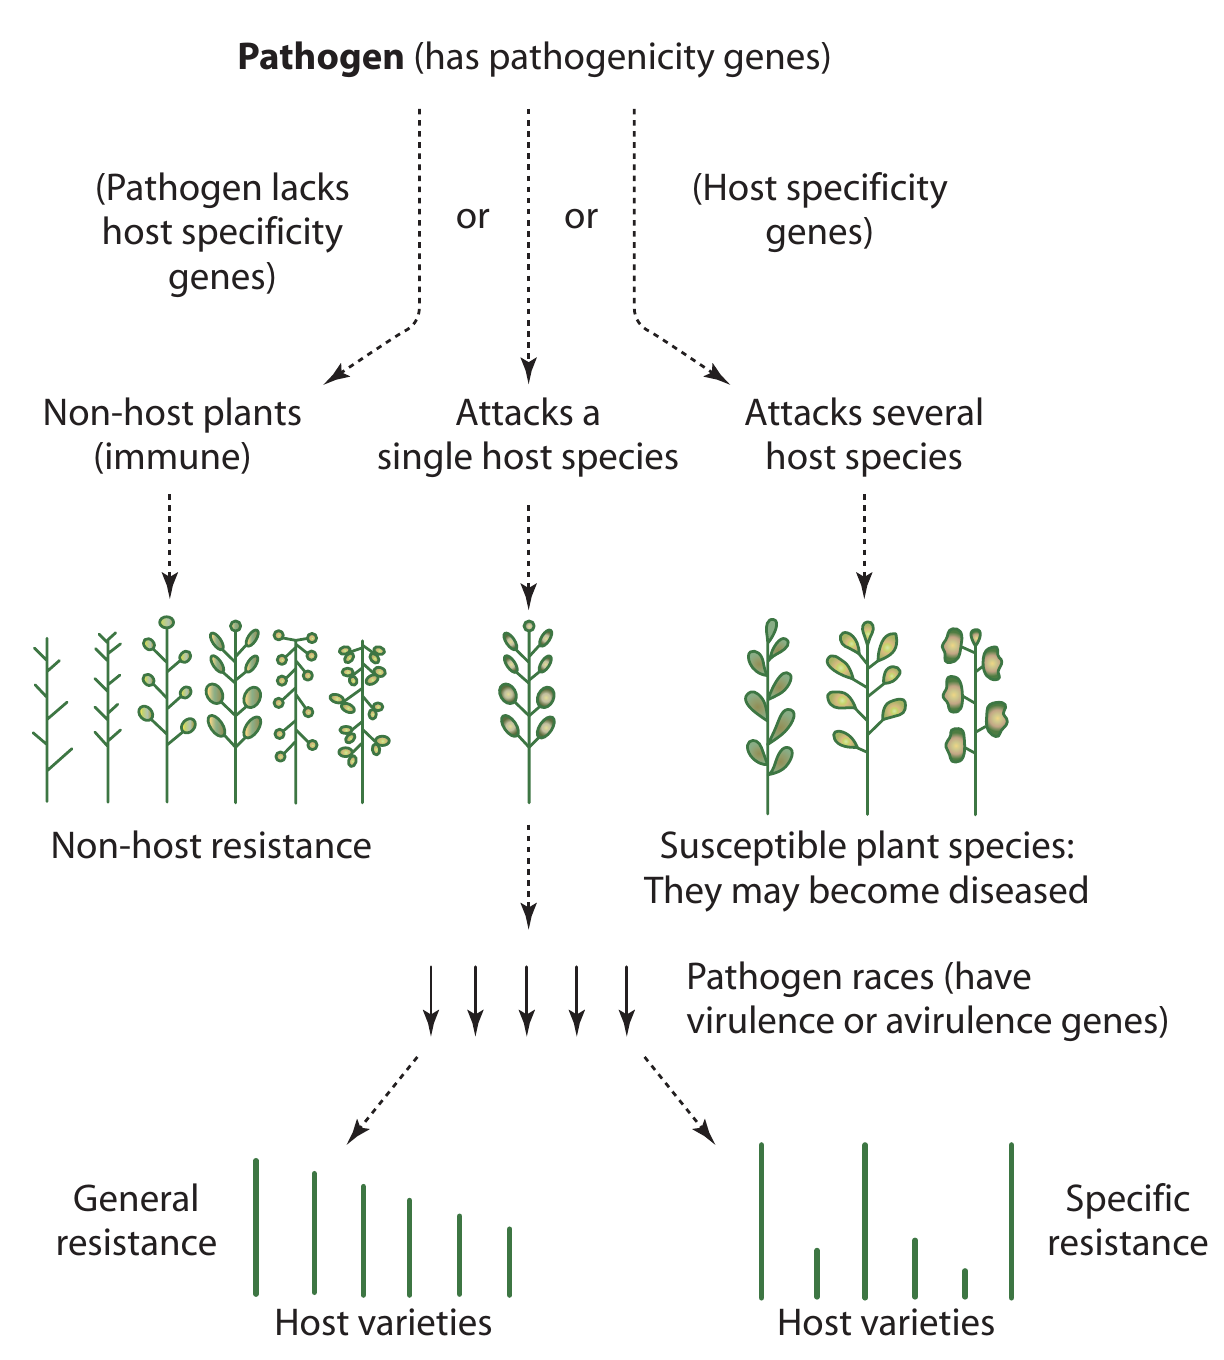
\includegraphics[width=0.7\linewidth]{../images/host_non_host} \caption{Gene interactions of a pathogen with its host and non-host plant}\label{fig:pathogen-host-non-host-interaction}
\end{figure}

\end{columns}
\end{frame}

\begin{frame}{}
\protect\hypertarget{section-1}{}
\begin{description}
\small
\item[Host range] List of plant species that can be exploited to be a natural enemy as source of nutrients.
\item[Generalists/polyphagous] Natural enemy with a wide host range.
\item[Specialits/oligophagous/monophagous] Natural enemy with a narrow host range or even single plant species.
\end{description}

\begin{itemize}
\tightlist
\item
  The complex of characters of a plant species that are responsible for
  making it a non-host to a certain potential natural enemy is non-host
  resistance.
\item
  No single individual plants of non-host species are susceptible to a
  natural enemy.
\end{itemize}
\end{frame}

\begin{frame}{}
\protect\hypertarget{section-2}{}
\small

\begin{itemize}
\tightlist
\item
  Non-host resistance (NHR) is largely modulated by PTI (discussed in
  Lecture: Introduction to Resistance Breeding)
\item
  NHR triggers multi-layered basal resistance mechanisms:

  \begin{itemize}
  \footnotesize
  \item peroxisome-based biosynthesis
  \item restriction of pathogen growth by nutrient limitation
  \item papilla formation
  \item callose and lignin deposition
  \end{itemize}
\item
  To contrast, genes involved in ETI pathways act on the basis of
  specific recognition, and develop hypersensitive response (HR)
  involving programmed cell death.
\item
  Many genes involved in NHR have multi-functional roles (including in)
  -- plant development
  (G-proteins\footnote[frame]{\scriptsize highly conserved heterotrimers proteins, mutation of which compromises NHR agaist fungal and bacterial pathogens}),
  stomatal regulation and plant metabolism.

  \begin{itemize}
  \footnotesize
  \item glycolate oxidase pathway
  \item proline dehydrogenase
  \end{itemize}
\item
  Both (above) enzymes modulate Reactive Oxygen Species (ROS) mediated
  signal transduction pathways in response to various environmental
  stresses! as well as providing NHR against bacterial pathogens.
\end{itemize}
\end{frame}

\begin{frame}{}
\protect\hypertarget{section-3}{}
\small

\begin{itemize}
\tightlist
\item
  NHR may be divided into 2 categories:

  \begin{itemize}
  \footnotesize
  \item Type I (does not show visible cell death symptoms)
  \item Type II (show localized hypersensitive response HR cell death, mediated through generation of ROS)
  \end{itemize}
\item
  NHR against pathogens of more closely related species can involve
  mechanisms more similar to host resistance

  \begin{itemize}
  \footnotesize
  \item maize resistance gene \textit{Rxo1} can recognize the rice bacterial streak pathogen
  \end{itemize}
\item
  Huanglongbing in citrus caused by vector-transmitted bacterial
  pathogen, \emph{Candidatus} spp. has been controlled through
  genetically modified alternative resistance gene from
  \emph{Arabidopsis thaliana}

  \begin{itemize}
  \scriptsize
  \item \textit{NPR1} gene transformed into sweet orange cultivars -- Hamlin and Valencia, and endogenous expression of \textit{AtNPR1} (targets signaling pathway for plant immunity) constitutively down-regulated\footnote[frame]{\scriptsize Refer to the article: The Arabidopsis AtNPR1 inversely modulates defense responses against fungal, bacterial, or viral pathogens while conferring hypersensitivity to abiotic stresses in transgenic rice, DOI: \url{https://doi.org/10.1094/mpmi-21-9-1215}}
  \end{itemize}
\end{itemize}
\end{frame}

\begin{frame}{}
\protect\hypertarget{section-4}{}
\small

\begin{itemize}
\tightlist
\item
  NHR resistance also sometimes provides broad spectrum resistance

  \begin{itemize}
  \footnotesize
  \item \textit{Rxo1} locus in maize confers resistance to all races of rice bacterial leaf streak pathogen \textit{Xanthomonas oryzae} pv. {oryzicola}.
  \item Tansgenic rice plants expressing \textit{Rxo1} showed strong resistance against \textit{X. oryzae} pv. {oryzicola}.
  \item This transgenic rice is resistant to another bacterial spot pathogen, \textit{Burkholderia andropogonis}.
  \end{itemize}
\item
  For breeding NHR mechanisms, steps are:

  \begin{itemize}
  \footnotesize
  \item screening of related species accessions (looking for susceptible individuals) among non-host species
  \item crossing and study of inheritance within non-host species to identify causal loci
  \item introgression of gene to host via hybridization with the non-host species, if possible
  \end{itemize}
\end{itemize}

\footnotesize

\begin{itemize}
\tightlist
\item
  Ideally, interfertile host as well as non-host species are hybridized
  and QTL mapping studies are conducted as in \textit{Bremia lactuca}.

  \begin{itemize}
  \scriptsize
  \item Lettuce downy mildew (causal: \textit{Bremia lactucae}) non-host \textit{Lactuca saligna} was crossed to host species \textit{L. sativa}, and backcross inbred lines were developed to stack alleles at four recessive NHR QTL\footnote[frame]{Refer to Genetic dissection of Lactuca saligna nonhost resistance to downy mildew at various lettuce developmental stages. DOI: \url{doi: 10.1111/j.1365-3059.2009.02066.x}}.
  \end{itemize}
\end{itemize}
\end{frame}

\hypertarget{hypersensitivity-and-partial-resistance}{%
\section{Hypersensitivity and partial
resistance}\label{hypersensitivity-and-partial-resistance}}

\begin{frame}{Hypersensitivity}
\protect\hypertarget{hypersensitivity}{}
\end{frame}

\begin{frame}{Partial resistance}
\protect\hypertarget{partial-resistance}{}
\end{frame}

\hypertarget{bibliography}{%
\section{Bibliography}\label{bibliography}}

\begin{frame}{References}
\protect\hypertarget{references}{}
\end{frame}




\end{document}
